\section{Internal gravity waves}
\subsection{The minimal mathematics version}

In a stably stratified fluid, consider a parcel of fluid. If the parcel is raised from its original position, then it will be heavier than the surrounding fluid, and will sink back down. If it is lowered, then buoyancy will push it back up. Thus density differences provide a restoring force to a parcel displaced vertically. 

Let $\rho(z)$ be the density of the fluid, with $z$ vertically upwards so that $\dod{\rho}{z} < 0$. If the parcel has volume $V$ and is displaced vertically by a height $H$, then the density difference between the parcel and the surrounding fluid is 
\begin{equation}
	\Delta\rho = \dod{\rho}{z} H
\end{equation}
and the downwards force on the parcel is therefore
\begin{equation}
	F = gV\Delta\rho = gV\dod{\rho}{z}H
\end{equation}
Meanwhile, the mass of the particle is 
\begin{equation}
	m = \rho V
\end{equation}
and so Newton's law $F = ma$ gives the acceleration
\begin{equation}
	a = \frac{g}{\rho}\dod{\rho}{z} H
\end{equation}
which is in the opposite direction to the displacement.

Assume that the fluid is \textit{Boussinesq}, so that density differences are small compared to a reference density $\rho_0$, and fluid accelerations are small compared to gravity. Then we make the approximation $\rho\approx\rho_0$ except when densities are multiplied by gravity. We define the \textit{buoyancy frequency} (or \textit{Brunt-V\"ais\"al\"a frequency}) $N$, such that
\begin{equation}
	N^2 = -\frac{g}{\rho_0}\dod{\rho}{z}.
\end{equation}
Then 
\begin{equation}
	a = -N^2 H
\end{equation}
so parcels of fluid execute oscillations with frequency $\omega = N$.

In the oceans, $N \approx 10^{-2}\mathrm{s^{-1}}$.

The above argument is not quite valid, because we cannot ignore continuity: we cannot simply displace a parcel of fluid without displacing some other fluid around it. Rather, we should consider displacing an entire slab of fluid and making it oscillate in its plane. But the same argument works.

Suppose a slab makes an angle $\theta$ to the vertical and is displaced by $d$ in that direction. Then the displacement in the vertical direction is $d\cos\theta$. A similar argument shows that the slab will execute oscillations with frequency
\begin{equation}
	\omega = N\cos\theta
	\label{igwdisprel-theta}
\end{equation}

\subsection{A more rigorous derivation}

We can derive the above more rigorously by starting from the governing equations of an incompressible inviscid fluid:
\begin{align}
	\divg\bs{u} &= 0\\
	\rho_t + \divg(\rho\bs{u}) &= 0\\
	(\rho\bs{u})_t +\divg(\rho\bs{u}\bs{u}) &= -\grad p + \rho\bs{g} 
\end{align}
which may also be written as 
\begin{align}
	\divg\bs{u} &= 0\\
	\rho_t + \bs{u}\cdot\grad\rho &= 0\\
	\rho (\bs{u}_t +\bs{u}\cdot\grad\bs{u}) &= -\grad p + \rho\bs{g}.
\end{align}
We perturb about the stationary stratified state, writing
\begin{align}
	\rho &= \bar{\rho}(z) + \rho' \\
	p &= \bar{p}(z) + p' 
\end{align}
and assume that the primed quantities and $\bs{u}$ are small. Then linearising the governing equations gives
\begin{align}
	\divg\bs{u} &= 0\\
	\dod{\bar{p}}{z} &= -g\bar{\rho} \\
	\rho_t &= -w\dod{\bar{\rho}}{z} \\
	\bar{\rho} \bs{u}_t &= -\grad p' - g\rho'\bs{e}_z. \label{govlin-mom}
\end{align}
For a Boussinesq fluid, $\rho\approx\rho_0$ except when multiplied by $g$, so (\ref{govlin-mom}) becomes
\begin{align}
	\bs{u}_t = -\frac{1}{\rho_0}\grad p' - \frac{g}{\rho_0} \rho' \bs{e}_z. \label{govlinbous-mom}
\end{align}
Take $\divg$(\ref{govlinbous-mom}) and use $\divg\bs{u} = 0$ to get
\begin{equation}
	\grad^2p' = -g\dpd{\rho'}{z}
\end{equation}
and then take $\grad^2$ of the $z$-component of (\ref{govlinbous-mom}) to get 
\begin{equation}
	\grad^2 w_t = -\frac{g}{\rho_0} (\rho'_{zz} - \grad^2 \rho')
\end{equation}
Differentiating with respect to time and using the equation for $\rho'_t$ gives
\begin{align}
	\grad^2w_tt &= \frac{g}{\rho_0} \left(\grad^2 - \dpd[2]{}{z}\right) (w\bar{\rho}_z) \\
			&\approx N^2 \left(\dpd[2]{}{z} - \grad^2\right) w
			\label{igw-govlin-w}
\end{align}
where the approximation applies for a Boussinesq fluid.

\paragraph{Plane wave eigenvalue problem}
For normal mode perturbations of the form
\begin{equation}
	w = \hat{w}\exp(i(\bs{k}\cdot\bs{x}-\omega t))
\end{equation}
where $\bs{k} = (k,l,m)$, we get the dispersion relation
\begin{equation}
	\omega^2 = N^2 \frac{k^2+l^2}{k^2+l^2+m^2}
	\label{igwldisprel-klm}
\end{equation}

How do we relate this to the argument with slabs, and recover (\ref{igwdisprel-theta})? We note that the slabs that we considered were lines of constant phase, i.e. of constant $\bs{k}\cdot\bs{x}$. So $\bs{k}$ is perpendicular to the slab. Hence if the slab makes an angle $\theta$ with the upwards vertical, then $\bs{k}$ makes an angle $\theta$ with the horizontal, and so
\begin{equation}
	\cos\theta = \frac{k^2+l^2}{k^2+l^2+m^2}
\end{equation}
as required. 

\paragraph{Evanescent waves}
Note that if $\omega > N$ then there are no real solutions to (\ref{igwdisprel-klm}). Rather, $(k,l,m)$ must be complex and have an imaginary component, which means $e^{i\bs{k}\cdot\bs{x}}$ decays exponentially as $\bs{x}$ increases in a certain direction. Such `waves' are called evanescent waves. A source which oscillates at a frequency $\omega$ will cause localised disturbances and energy is not carried away.

\subsection{Wave velocities}

From the dispersion relation, we obtain the phase and group velocities in the usual way:
\begin{align}
	\bs{c}_p &= \frac{\omega}{|\bs{k}|} \hat{\bs{k}} \\
		&= \frac{N}{k}\cos\theta \hat{\bs{k}} \\
		&= N \sqrt{\frac{k^2+l^2}{k^2+l^2+m^2}} (k,l,m)
\end{align}
and
\begin{align}
	\bs{c}_g &= \dpd{\omega}{\bs{k}} \\
		&= -N \sin\theta \dpd{\theta}{\bs{k}}\\
		&=\frac{N}{|\bs{k}|^3 \sqrt{k^2+l^2}} (km^2,lm^2,-(k^2+l^2)m)
\end{align}

Note that 
\begin{equation}
	\bs{c}_p\cdot\bs{c}_g = 0
\end{equation}
so the phase and group velocities are perpendicular; and note that the group and phase velocities have $z$-components in opposite directions. See figure \ref{fig:igw-wave-vels}.

The phase velocity is the velocity at which crests move, or more abstractly the velocity at which phase is advected. The group velocity is the velocity with which wavepackets propagate, and can be interpreted as a rate and direction of energy transfer. The group velocity makes an angle $\theta$ with the vertical. 

\begin{figure}
\begin{center}
	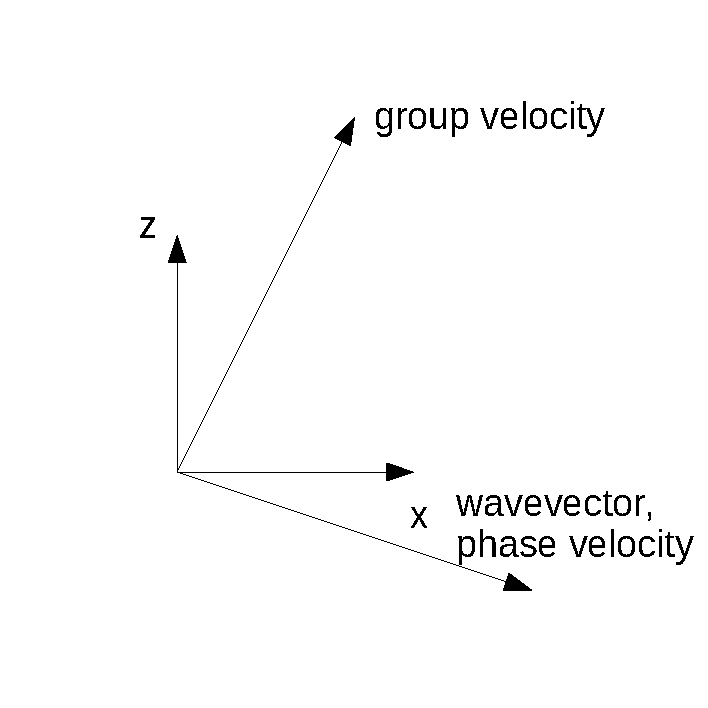
\includegraphics[width=8cm]{igw-wave-vels.pdf}
	\caption{The geometric relationship between phase velocity, group velocity and wavevector.}
	\label{fig:igw-wave-vels}
\end{center}
\end{figure}

\subsection{Motion of fluid particles}

If $\bs{u} = (u,0,w)$ and 
\begin{align}
	u&=\hat{u} \exp(i(\bs{k}\cdot\bs{x} - \omega t)) \\
	w&=\hat{w} \exp(i(\bs{k}\cdot\bs{x} - \omega t)) \\
\end{align}
then $\divg\bs{u}=0$ gives
\begin{equation}
	\hat{u} = -\frac{m}{k}\hat{w}
\end{equation}
which tells us that fluid particles oscillate parallel to the group velocity and perpendicularly to the wavevector. We can obtain the displacements by integrating with respect to time, or equivalently by dividing by $-i\omega$. 

\subsection{Equipartition of energy}

Dotting (\ref{govlinbous-mom}) with $\bs{u}$ and some manipulation gives us
\begin{equation}
	\dpd{}{t}\left(\frac{1}{2}\rho_0 \bs{u}^2 + \frac{1}{2}\frac{g^2}{\rho_0N^2}\rho'^2\right) + \divg(p'\bs{u}) = 0,
\end{equation}
the equation of conservation of energy. We identify $ \frac{1}{2}\rho_0 \bs{u}^2 $ as kinetic energy density and $\frac{1}{2}\frac{g^2}{\rho_0N^2}\rho'^2$ as potential energy density. (Energy density is energy per unit volume.)

For normal modes, we can calculate time-averages, and find that 
\begin{equation}
\langle\text{kinetic energy density}\rangle = \langle\text{potential energy density}\rangle
\end{equation}
%TODO

Note that we must take real parts before multiplying together any quantities. 

\subsection{Oscillating cylinders}

Suppose a cylinder (or any other object) is suspended in a stratified medium. At time $t=0$, it is impulsively started to oscillate at frequency $\omega<N$. The impulsive start of the cylinder generates an entire spectrum of transient wave modes, which generates IGWs propagating at different values of $\theta$. After some time, when the transients have decayed, we see a single mode of IGWs propagating at $\theta = \cos^{-1} (\omega/N)$ to the vertical. 

\subsection{Reflexions}
\subsubsection{Properties of reflected beams}

\begin{figure}
\begin{center}
	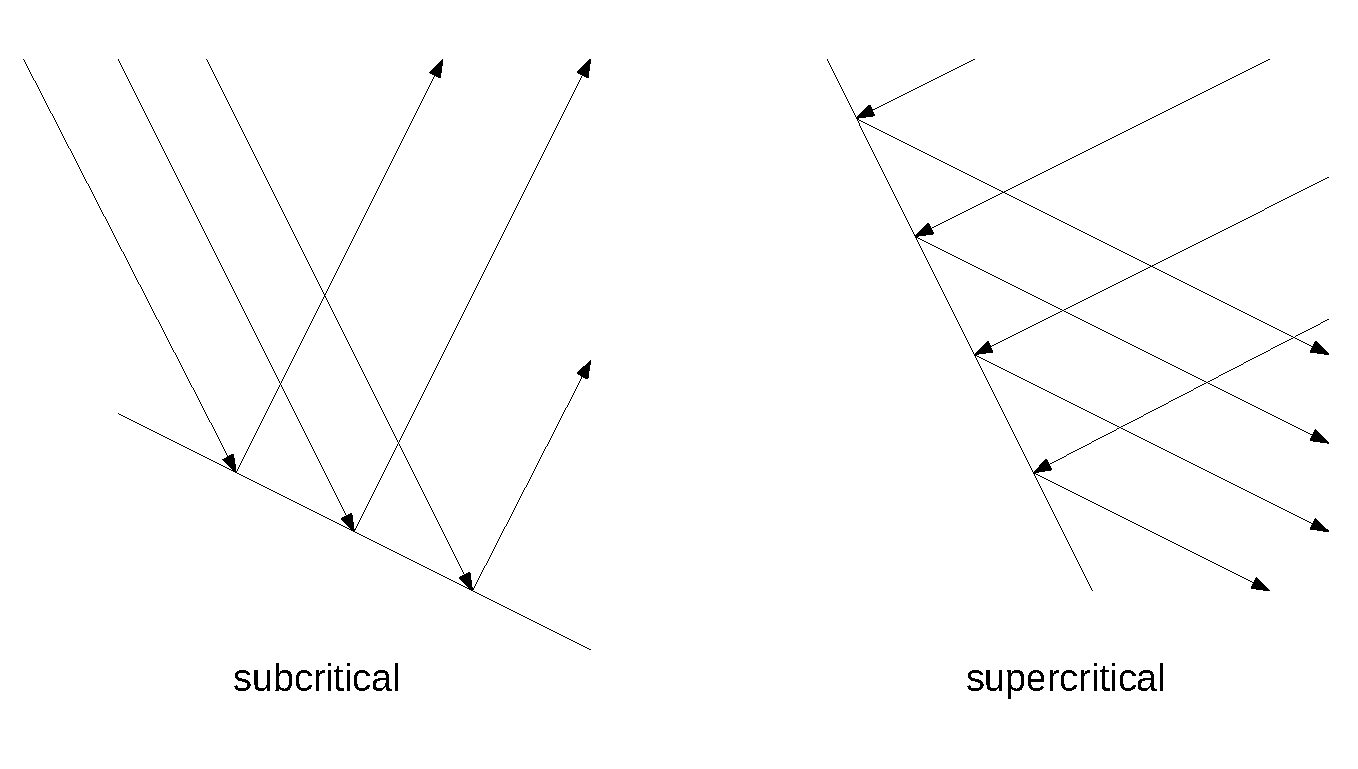
\includegraphics[width=14cm]{super-and-sub-critical.pdf}
	\caption{Super- and sub-critical reflexions.}
	\label{fig:supersubcrit}
\end{center}
\end{figure}


At a boundary, the normal velocity component must be continuous. For a rigid stationary boundary, this means that the normal velocity component must vanish.

Suppose $z=0$ is a rigid stationary boundary, with a plane wave incident from $z>0$. What is the reflected wave? We have 
\begin{align}
	w &= w_I + w_R \\
	w_I &= \hat{w}_I \exp(i(\bs{k}_I\cdot\bs{x} - \omega t)) \\
	w_R &= \hat{w}_I \exp(i(\bs{k}_R\cdot\bs{x} - \omega t));
\end{align}
the two waves must have the same $\omega$ and $k_I = k_R$; the boundary condition gives $\hat{w}_I + \hat{w}_R = 0$. And causality implies that $m_R = -m_I$. 

When a plane wave reflects off a flat boundary which is not horizontal, then the incident and reflected waves make the same angle (but reflected) with the vertical or horizontal, so that they have the same $\omega = N\cos\theta$. (Note that for IGWs, $\theta$ is the angle between a wave's direction and the vertical.) In general, the angle of incidence and angle of reflexion are not equal. Depending on how the angle of the incident wave compares with the slope of the boundary, one of two things may happen: see Figure \ref{fig:supersubcrit}. 

From Figure \ref{fig:supersubcrit} we can see that reflexions change the wavenumber of the wave and can act to focus or defocus the rays, depending on direction. Let $\alpha$ be the angle that the plane boundary makes with the vertical. We define the quantity 
\begin{equation}
	\gamma  =  \frac{\sin(\alpha-\theta)}{\sin(\alpha+\theta)}
\end{equation}
to characterise the focusing power of a reflexion. 

After a lot of manipulation, we can show that focusing reflexions change the amplitude and wavenumber according to
\begin{align}
	k_R  &= \gamma k_I \\
	A_R &= \gamma A_I 
\end{align}
and that defocusing reflexions have the opposite effect:
\begin{align}
	k_R  &= \gamma^{-1} k_I \\
	A_R &= \gamma^{-1} A_I.
\end{align}

\subsubsection{Energy density upon reflexion}

The energy density per unit wavelength is 
\begin{equation}
	\tilde{E} \sim \lambda A^2.
\end{equation}
After a focusing reflexion, $\lambda$ is divided by $\gamma$ but $A$ is multiplied by $\gamma$, so $\tilde{E}$ is multiplied by $\gamma$. Hence the energy density per wavelength is increased after a focusing reflexion. 

The energy density per unit length is 
\begin{equation}
	\hat{E} = \frac{1}{\lambda} \tilde{E}
\end{equation}
and so $\hat{E}$ is multiplied by $\gamma^2$ after a focusing reflexion.

\subsubsection{Subcritical and supercritical reflexions}

In a subcritical reflexion, the boundary has a shallower slope than the wave ($\theta < \alpha$), and the vertical propagation of the wave is reversed by the reflexion. The horizontal direction of propagation is maintained.

In a supercritical reflexion, $\theta > \alpha$ and the vertical direction of propagation is maintained but the horizontal direction is reversed. 

When $\theta$ and $\alpha$ are very similar, then $\gamma$ becomes very large. So waves will have very large amplitudes, and nonlinear effects and viscosity become important. 

\subsection{Ray tracing}

Since the frequency is preserved upon reflexion, the angle to the vertical $\theta$ is conserved, so waves tend to propagate along well-defined rays. Depending on the shape of the domain and its boundaries, repeated reflexions can lead to trapping, to amplitudes increasing, and eventually to wave-breaking. Nonlinear effects become important if the amplitude of waves is increased sufficiently.

We must take note of causality to determine which direction is appropriate.

\subsection{Wave attractors}
\subsubsection{Rectangular basins}
\subsubsection{Trapezoidal basin}
\subsubsection{More complex geometries}
\subsubsection{Energy spectrum for attractor}

\subsection{Decay along a beam}

Here we will derive the behaviour for a beam in a viscous fluid with constant kinematic viscosity $\nu$. The linearised equations are now
\begin{align}
	\dpd{u}{t} + \frac{1}{\rho_0}\dpd{p}{x} &= \nu\grad^2 u \\
	\dpd{w}{t} + \frac{1}{\rho_0}\dpd{p}{z} - b &= \nu\grad^2 w \\
	\dpd{b}{t} + N^2w &= 0 \\
	\divg\bs{u} &= 0
\end{align}
where 
\begin{equation}
	b = \displaystyle\frac{-g(\rho-\rho_0)}{\rho_0}
\end{equation}
is the buoyancy. 

Introduce a streamfunction $\psi$ such that $(u,w) = (-\psi_z, w= \psi_x)$. Then some cross-differentiation eliminates $p$ and $b$ to give
\begin{equation}
	\grad^2 \psi_{tt} + N^2 \psi_{xx} = \nu\grad^4 \psi_t.
	\label{igw-damped}
\end{equation} 

The $\nu\grad^4\psi_t$ term acts to damp waves. We could look for plane-wave solutions to (\ref{igw-damped}) in the usual way, and obtain the dispersion relation
\begin{equation}
	\omega^2 + i\nu(k^2+m^2) - N^2\cos^2\theta = 0
	\label{igwdisprel-damped}
\end{equation}
where $\cos\theta = k/|\bs{k}|$ as usual. Given $(k,m)$, we could solve (\ref{igwdisprel-damped}) for $\omega$. 

But often we are more interested in the spatial decay of a beam that is generated by oscillations at a fixed $\omega$. We expect that the beam would still propagate in the direction $\theta = \cos^{-1} (\omega/N)$, but with a decaying amplitude.

\subsection{Reflexions from rough topology}

\subsubsection{Subcritical reflexion from a sinusoidal}
\subsubsection{Supercritical reflexions from a sinusoidal}

\subsection{Non-linear stratification}

If $N$ is not constant but varies with $z$ (say), then waves will not follow straight paths but will refract. If $N$ varies very slowly with $z$, over lengthscales much larger than a wavelength, then the WKB method can be used to find the trajectory of a wave. We use the fact that $\omega = N(z)\cos\theta$ is constant along any beam to determine $\theta$, the angle between the beam and the vertical. 



\subsection{Leewaves}

When a medium flows past an obstacle and waves are formed in the wake, it is possible to get standing waves (also known as stationary waves). When standing IGWs occur in the atmosphere as a wind flows past obstacles such as mountains, these are known as leewaves.

\subsubsection{Kelvin ship waves}

As an aside to introduce standing waves, we consider a ship moving with velocity $\bs{U} = U\bs{e}_x$ in deep water. The surface waves have a dispersion relation
\begin{equation}
\omega^2 = g|\bs{k}|
\end{equation}
and phase
\begin{equation}
	\phi = \bs{k}\cdot\bs{x} - \omega t.
\end{equation}
Let $\bs{x}'$ denote a position vector relative to the ship, so that $\bs{x}' = \bs{x} - \bs{U}t$. Then
\begin{equation}
	\phi = \bs{k}\cdot\bs{x}' + (\bs{k}\cdot\bs{U} - \omega) t.
\end{equation}
Hence waves that are stationary in the frame of the ship have
\begin{align}
	\bs{k}\cdot\bs{U} &= \omega \\
	U\cos\theta &= |\bs{c}_g|
\end{align}
where, in this section, $\theta$ is the angle between $\bs{U}$ and $\bs{k}$. 

For these waves, $\bs{c}_g$ and $\bs{c}_p$ are parallel, and $|\bs{c}_g| = \frac{1}{2} |\bs{c}_p| = \frac{1}{2}U\cos\theta$. This is the speed at which wave packets travel. Some geometry then tells us the shape that these waves make behind the ship.

In shallow water, surface waves are not dispersive and such stationary waves are not seen.

\subsubsection{Extended range of hills}

Now we consider leewaves, i.e. stationary atmospheric IGWs as a wind of speed $U$ flows, from left to right, over a sinusoidal mountain range which has wavelength $\lambda_T$ and so topographical wavenumber $k_T = 2\pi/\lambda$. 

An observer in the frame of the mountains sees the leewaves as having a constant phase. The frequency of the forcing must therefore be
\begin{equation}
	\omega = k_T U = \frac{2\pi U}{\lambda_T}
\end{equation}
and the wave crests make an angle $\theta = \cos^{-1} (\omega/N)$ with the vertical. The phase velocity is aligned with the wave crests, so that the observer sees the waves as being stationary.

We move to a frame moving with the wind, in which the mountains are moving with speed $U$ to the left. This does not change the angle between the wave crests and the vertical. But in the new frame the group velocity is $\bs{c}'_g = \bs{c}_g - \bs{U}$, and is aligned with the crests. 

\subsubsection{Causality}

\subsection{Shear flows}

\subsubsection{Sheared base state}

Suppose the background stratified fluid is not stationary but has velocity $\bs{U} = (U(z),0,0)$. Linearising the full governing equations of motion about this base state by writing $\bs{u} = \bs{U} + (u',v',w')$, and a lot of manipulation to eliminate everything apart from $w'$, eventually gives
\begin{equation}
	\left(\dpd{}{t} + U\dpd{}{x}\right)^2 \grad^2 w' + N^2 \dpd[2]{w'}{x} - U''\left(\dpd{}{t} + U\dpd{}{x}\right)\dpd{w'}{x} = 0.
\end{equation}
Note that this reduces to \ref{igw-govlin-w} if $U\equiv0$. If $U$ is constant, then a change of frame would recover \ref{igw-govlin-w} as expected.

For flows which are steady (in this frame of reference), we have
\begin{equation}
	\dpd[2]{}{x} \grad^2 w' + \left( \frac{N^2}{U^2} - \frac{U''}{U} \right)\dpd[2]{w'}{x} = 0.
\end{equation}
Integrating twice with respect to $x$ then gives
\begin{equation}
	\grad^2 w' + \left( \frac{N^2}{U^2} - \frac{U''}{U} \right) w' = 0.
\end{equation}

If $U$ and $N$ are constant, or very slowly varying, then we can search for plane wave solutions
\begin{equation}
	w' = w_0 e^{i(kx+mz)}
\end{equation}
which satisfy
\begin{equation}
	-(k^2 + m^2) + \frac{N^2}{U^2} = 0
\end{equation}
or $|\bs{k}| = N/U$ as before. Note that this is also true whenever
\begin{equation}
	\frac{N^2}{U^2} - \frac{U''}{U} 
\end{equation}
is constant.

\subsubsection{Ray tracing in a shear flow}

When the length scale over which $U$ and $N$ change is much larger than the wavelength of internal waves, we can consider the important wave properties as being instantaneous in the local state of the background flow. This is the WKB approximation. Rays follow the group velocity relative to the fluid. However, in our frame of reference the waves appear stationary, and so the phase velocity must be parallel to the wave crests and the group velocity antiparallel with the wavenumber vector. We can thus take the trajectory of a wave propagating with the mean flow as
\begin{equation}
	\dod{z}{x} = \frac{c_{gz}}{U - c_{gx}} = \frac{m}{k}
\end{equation}
where $\bs{c}_g$ is the group velocity relative to the fluid.

Recalling that $k^2 + m^2 = N^2 / U^2$, and assuming that $k$ is conserved along the ray and $U''/U \ll N^2 /U^2$, then
\begin{equation}
	m^2 = \frac{N^2}{U^2} - k^2
\end{equation}
and so 
\begin{equation}
	\dod{z}{x} = \left(\left(\frac{N}{kU}\right)^2 - 1\right)^{1/2}.
\end{equation}
Waves cannot propagate through a level where $kU/N = 1$.

In the atmosphere, $U/N$ tends to increase with height as $U$ increases.

\subsubsection{*Three-dimensional forcing}
\subsubsection{*Effect of viscosity}
\subsubsection{*Blocking}

\subsection{Columnar modes}
\subsection{*Stokes drift in internal waves}
\subsection{Resonant triads}